\documentclass[12pt, a4paper]{article}
\usepackage[utf8]{inputenc}
\usepackage{amsmath, amssymb, amsthm, amsfonts}
\usepackage{CJKutf8}
\usepackage[margin=1in]{geometry}
\usepackage{tikz}
\newtheorem{lemma}{Lemma}
\newcommand{\g}{\mathfrak{g}}
\newcommand{\h}{\mathfrak{h}}
% 重新定义 solution 环境，保留标识并在末尾留出 8cm 空白
\newenvironment{solution}
  {\paragraph{\textit{Solution:}}\par\medskip}
  {\hfill$\blacksquare$\vspace{0.1cm}}

\title{Lie Theory:Assignment 4}
\author{
    \begin{CJK*}{UTF8}{gbsn}
    钟皓宇 (12533556)
    \end{CJK*}
}
\date{\today}

\begin{document}

\maketitle


\section*{Problem 1}
Prove that $\Phi^\vee$ is a root system in $E$, whose Weyl group is naturally isomorphic to $\mathcal{W}$; show also that $\langle \alpha^\vee, \beta^\vee \rangle = \langle \beta, \alpha \rangle$, and draw a picture of $\Phi^\vee$ in the cases $A_1, A_2, B_2, G_2$.
\begin{solution}
  R1 holds for $\Phi^\vee$.
  Since $\Phi$ is finite then $\Phi^\vee$ is also finite. Hence $\Phi$ does not contain zero implies that $\Phi^\vee$ also does not contain zero.
  $\Phi$ and $\Phi^\vee$ can be linearly represented for each other, it implies that $\Phi^\vee$ spans $E$.
  R2 holds for $\Phi^\vee$ for the reason that the dual operator just change the norm but not change the angle. To see that we have calculation:
  \begin{align*}
    \cos\theta_{\alpha^\vee,\beta^\vee}= \frac{(\alpha^\vee,\beta^\vee)}{\|\alpha^\vee\|\cdot \|\beta^\vee\|} = \frac{4(\alpha,\beta)}{\|\alpha\|^2\cdot \|\beta\|^2}\cdot \frac{\|\alpha\|\cdot \|\beta\|}{4} =\frac{(\alpha,\beta)}{\|\alpha\|\cdot \|\beta\|}=  \cos\theta_{\alpha,\beta},
  \end{align*}
  for arbitrary elements $\alpha,\beta\in \Phi$. Hence, we find that $(-\alpha)^\vee=-\alpha^\vee$.
  Therefore, R2 holds.
  For R3, we see that 
  \begin{align*}
    \sigma_{\alpha^\vee}(\beta^\vee) = \beta^\vee -\frac{2(\beta^\vee,\alpha^\vee)}{\|\alpha^\vee\|^2}\alpha^\vee 
  \end{align*}
  Since $\alpha^\vee/\|\alpha^\vee\|=\alpha/\|\alpha\|$ we obtain that 
  \begin{align*}
     \sigma_{\alpha^\vee}(\beta^\vee) = \sigma_{\alpha}(\beta^\vee)=\frac{2\beta}{\|\beta\|^2} - \frac{4(\beta,\alpha)}{\|\beta\|^2 \cdot \|\alpha\|^2} \alpha = \frac{2}{\|\beta\|^2}\sigma_{\alpha}(\beta).
  \end{align*}
  Because $\sigma_{\alpha}$ is a reflection, it does not change the norm. Moreover, $\sigma_\alpha$ leaves $\Phi$ invariant. Then we find that 
  \begin{align*}
    \sigma_{\alpha^\vee}(\beta^\vee) = (\sigma_\alpha(\beta))^\vee \in \Phi^\vee.
  \end{align*} 
  It shows that $\sigma_{\alpha^\vee}$ leaves $\Phi^\vee$ invariant. 
  R4 is also true. Because 
  \begin{align*}
    \langle \beta^\vee,\alpha^\vee \rangle = (\beta^\vee, (\alpha^\vee)^\vee)=(\beta^\vee,\alpha) = \langle \alpha,\beta \rangle \in \mathbb{Z}.
  \end{align*}
  Therefore, we obtain that $\Phi^\vee$ is also a root system.
  In the previous discussion, we can see that $\sigma_{\alpha} = \sigma_{\alpha^\vee}$. Therefore, the Weyl groups of $\Phi$ and $\Phi^\vee$ are the same subgroup of $\text{GL}(E)$ since they share the same generators.
  The picture of $\Phi^\vee$ as follow.
  \begin{figure}[htbp]
    \centering
    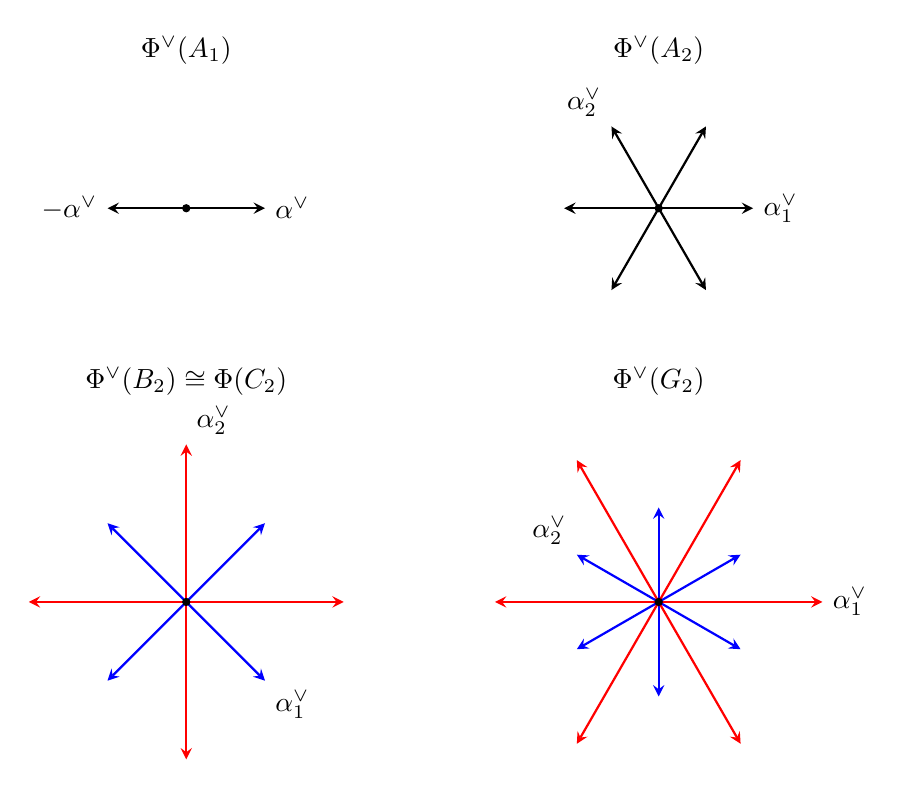
\begin{tikzpicture}[>=stealth, thick]
        
        % ====================
        % 1. A1 Dual Root System
        % ====================
        \begin{scope}[xshift=0cm, yshift=0cm]
            \node at (0, 2) {$\Phi^\vee(A_1)$};
            
            \draw[->] (0,0) -- (1,0) node[right] {$\alpha^\vee$};
            \draw[->] (0,0) -- (-1,0) node[left] {$-\alpha^\vee$};
            
            \fill (0,0) circle (1.5pt);
        \end{scope}

        % ====================
        % 2. A2 Dual Root System
        % ====================
        \begin{scope}[xshift=6cm, yshift=0cm]
            \node at (0, 2) {$\Phi^\vee(A_2)$};
            
            \foreach \a in {0, 60, 120, 180, 240, 300} {
                \draw[->] (0,0) -- (\a:1.2);
            }
            
            \node[right] at (0:1.2) {$\alpha_1^\vee$};
            \node[above left] at (120:1.2) {$\alpha_2^\vee$};
            
            \fill (0,0) circle (1.5pt);
        \end{scope}

        % ====================
        % 3. B2 Dual Root System (Isomorphic to C2)
        % ====================
        \begin{scope}[xshift=0cm, yshift=-5cm]
            \node at (0, 2.8) {$\Phi^\vee(B_2) \cong \Phi(C_2)$};
            
            % Short roots (diagonals)
            \foreach \x/\y in {1/1, -1/1, -1/-1, 1/-1} {
                \draw[->, blue] (0,0) -- (\x,\y);
            }
            % Long roots (axes)
            \foreach \x/\y in {2/0, -2/0, 0/2, 0/-2} {
                \draw[->, red] (0,0) -- (\x,\y);
            }
            
            \node[below right] at (1,-1) {$\alpha_1^\vee$}; % Simple root 1 (short)
            \node[above right] at (0,2) {$\alpha_2^\vee$};  % Simple root 2 (long)
            
            \fill (0,0) circle (1.5pt);
        \end{scope}

        % ====================
        % 4. G2 Dual Root System
        % ====================
        \begin{scope}[xshift=6cm, yshift=-5cm]
            \node at (0, 2.8) {$\Phi^\vee(G_2)$};
            
            % Short roots (Angles: 30, 90, 150, 210, 270, 330)
            \foreach \a in {30, 90, 150, 210, 270, 330} {
                \draw[->, blue] (0,0) -- (\a:1.2);
            }
            % Long roots (Angles: 0, 60, 120, 180, 240, 300)
            % Length ratio is sqrt(3) approx 1.732. So 1.2 * 1.732 = 2.08
            \foreach \a in {0, 60, 120, 180, 240, 300} {
                \draw[->, red] (0,0) -- (\a:2.08); 
            }
            
            \node[right] at (0:2.08) {$\alpha_1^\vee$};     % Simple root 1 (long)
            \node[above left] at (150:1.2) {$\alpha_2^\vee$}; % Simple root 2 (short)
            
            \fill (0,0) circle (1.5pt);
        \end{scope}

    \end{tikzpicture}
    \caption{The dual root systems $\Phi^\vee$ for $A_1, A_2, B_2, G_2$.}
    \label{fig:dual_root_systems}
\end{figure}
\end{solution}



\section*{Problem 2}
Let $\Phi^\vee$ be the dual system of $\Phi, \Delta^\vee = \{\alpha^\vee \mid \alpha \in \Delta\}$. Prove that $\Delta^\vee$ is a base of $\Phi^\vee$. [Compare Weyl chambers of $\Phi$ and $\Phi^\vee$.]
\begin{solution}
  Since the dual operator does not change the hyperplane. Explicitly, we say $P_{\alpha}=P_{\alpha^\vee}$.
  It implies that $\Phi$ and $\Phi^\vee$ share the same Weyl chambers. 
  Suppose that $\Delta=\{\alpha_1,\dots,\alpha_n\}$, then it define a Weyl chamber 
  \begin{align*}
    C(\Delta) = \{x\in E\mid (x,\alpha_i)>0\text{ for }i=1,\dots,n\}.
  \end{align*}
  Equivalently, we obtain that 
  \begin{align*}
    C(\Delta) = \{x\in E\mid (x,\alpha^\vee_i)>0\text{ for }i=1,\dots,n\}.
  \end{align*}
  According to our textbook, $C(\Delta)$ as the Weyl chamber of $\Phi^\vee$ can be uniquely determined by roots $\{\beta_1^\vee,\dots,\beta_n^\vee\}$ such that 
    \begin{align*}
    C(\Delta) = \{x\in E\mid (x,\beta^\vee_i)>0\text{ for }i=1,\dots,n\},
  \end{align*}
  and $\{\beta_i\}$ form a base. It implies that $\Delta^\vee=\{\beta_1,\dots,\beta_n\}$ and thus $\Delta^\vee$ is a base of $\Phi^\vee$.
\end{solution}



\section*{Problem 3}
Given $\Delta = \{\alpha_1, \dots, \alpha_l\}$ in $\Phi$, let $\lambda = \sum_{i=1}^l k_i \alpha_i$ ($k_i \in \mathbf{Z}$, all $k_i \ge 0$ or all $k_i \le 0$). Prove that either $\lambda$ is a multiple (possibly 0) of a root, or else there exists $\sigma \in \mathcal{W}$ such that $\sigma \lambda = \sum_{i=1}^l k'_i \alpha_i$, with some $k'_i > 0$ and some $k'_i < 0$. [Sketch of proof: If $\lambda$ is not a multiple of any root, then the hyperplane $P_\lambda$ orthogonal to $\lambda$ is not included in $\bigcup_{\alpha \in \Phi} P_\alpha$. Take $\mu \in P_\lambda - \bigcup_{\alpha \in \Phi} P_\alpha$. Then find $\sigma \in \mathcal{W}$ for which all $(\alpha_i, \sigma \mu) > 0$. It follows that $0 = (\lambda, \mu) = (\sigma \lambda, \sigma \mu) = \sum k'_i (\alpha_i, \sigma \mu)$.]

\begin{solution}
  We use the notation of hint and follow its discussion.  
  Let $C(\Delta)$ denote the fundamental Weyl chamber determined by $\Delta$. Since $\mu$ is a regular vector, equivalently, we say there exists a Weyl chamber containing $\mu$.
  According to our textbook, the Weyl group acts transitively on Weyl chambers, then there exists $\sigma\in \mathcal{W}$ such that $\sigma(\mu)\in C(\Delta)$.
  It implies that $(\alpha_i,\sigma(\mu))>0$ for all $i=1,\dots,l$. Because we have
  \begin{align*}
    0 = (\lambda, \mu) = (\sigma \lambda, \sigma \mu) = \sum k'_i (\alpha_i, \sigma \mu).
  \end{align*}
  The positivity of $(\alpha_i, \sigma \mu)$ implies the set $\{k_i'\}$ must contains negative and positive integers. Otherwise, it must equal to $\{0\}$ meaning that $\lambda=0$. It is impossible, since in this case, $\lambda = 0\cdot \alpha_1$ is a multiple of a root. 
\end{solution}


\section*{Problem 4}
Prove that if $\alpha, \beta$ are roots, $\beta \neq \pm \alpha$, $k$ is a real number and $\beta + k \alpha$ is a root, then $k$ is an integer.
\begin{solution}
  Let $\gamma$ denote $\beta+k\alpha$
  First, we consider that 
  \begin{align*}
    \langle \gamma,\alpha \rangle = 2k+\langle \beta,\alpha\rangle  \in \mathbb{Z}.
  \end{align*}
  It requires that $k\in (1/2)\cdot \mathbb{Z}$. Hence, we consider 
  \begin{align*}
    \langle \gamma,\beta \rangle = 2 + k\langle \alpha,\beta\rangle \in \mathbb{Z}.
  \end{align*}
  Suppose that $k=m/2$ is not an integer, then we must have $\langle \alpha,\beta\rangle \in 2\mathbb{Z}$.
  Hence, since $-k\alpha = \beta - \gamma$ we consider
  \begin{align*}
    -k \langle \alpha, \gamma \rangle = \langle \beta, \gamma \rangle - 2 \in \mathbb{Z}
  \end{align*}
  implies that $\langle\alpha,\gamma\rangle \in 2\mathbb{Z}$. Similarly, we consider $k\alpha = \gamma - \beta$  and 
  \begin{align*}
    k\langle \alpha, \beta \rangle  = \langle \gamma, \beta \rangle - 2 \in \mathbb{Z}.
  \end{align*}
  It implies that $\langle \alpha, \beta \rangle\in 2\mathbb{Z}$. Since we have $\langle \alpha, \beta \rangle\in\{0, \pm 1, \pm 2, \pm 3\}$, then $\langle \alpha, \beta \rangle$ must be $0$ or $\pm 2$.
  If $\langle \alpha, \beta \rangle = 0$, then we have $\langle \gamma,\beta\rangle = 2$.
  It means that $\langle \beta,\gamma\rangle = 1$ and $(\gamma, \gamma) = 2(\beta, \beta)$. Moreover, we have 
  $$(\gamma, \gamma) = (\beta + k\alpha, \beta + k\alpha) = (\beta, \beta) + k^2(\alpha, \alpha) + 2k(\alpha, \beta)$$
  It implies that $(\beta, \beta) = k^2(\alpha, \alpha)$.
  Since we have
  $$\langle \alpha, \gamma \rangle = \frac{2(\alpha, \beta + k\alpha)}{(\gamma, \gamma)} = \frac{2k(\alpha, \alpha)}{2(\beta, \beta)} = \frac{k(\alpha, \alpha)}{k^2(\alpha, \alpha)} = \frac{1}{k} = \frac{2}{m}\in 2\mathbb{Z}$$
  we obtain that $m=\pm 1$. If $m=1$, then we have 
  \begin{align*}
    (\alpha, \alpha) = 4(\beta, \beta) = 2(\gamma, \gamma)
  \end{align*}
  and $s_\gamma(\beta) = -\frac{1}{2}\alpha\in \Phi$ which is the multiple of $\alpha$. It is impossible.
  If $m=-1$, by the same reason, we have $s_\gamma(\beta) = \frac{1}{2}\alpha \in \Phi$, which is also impossible.
  Suppose that $\langle \alpha, \beta \rangle = \pm 2$ then we have 
  \begin{align*}
    (\alpha, \alpha) = 2(\beta, \beta) \quad 
    \langle \beta, \alpha \rangle = \pm 1 \quad 
    (\alpha, \beta) = \pm (\beta, \beta)
  \end{align*}
  Hence, we have 
  $$(\gamma, \gamma) =  (1  \pm 2k + 2k^2)(\beta, \beta).$$
  Moreover, we obtain that 
  $$\langle \alpha, \gamma \rangle = \frac{\pm 2 + 2m}{1 \pm m + m^2/2} \in 2\mathbb{Z}$$.
  Rewrite this formula, we obtain that 
  \begin{align*}
    \frac{2(m\pm 1)}{(m\pm 1)^2+1}\in \mathbb{Z}.
  \end{align*}
  Since $m$ is odd, then $x = m\pm 1$ is even. The upper formula is equal to say 
  \begin{align*}
    \frac{2x}{x^2+1}\in\mathbb{Z}
  \end{align*}
  If $|x|\ge 2$, then we find that $|\frac{2x}{x^2+1}|<1$, it implies that $x=0$ and thus $m=\mp 1$. Then we find that 
  \begin{align*}
    (\gamma, \gamma) = (1 - 1 + 1/2)(\beta, \beta) = \frac{1}{2}(\beta, \beta).
  \end{align*}
  It implies that $(\alpha, \alpha) = 2(\beta, \beta) = 4(\gamma, \gamma)$ which is impossible. 
  Therefore, $k$ must be an integer.
\end{solution}
\end{document}